\section{Experimento de Doble Rendija de Young}

Este experimento consiste en aislar dos rayos de una fuente de luz
y fijar un punto distante de esta fuente, para así poder medir el
efecto de la interferencia de las dos ondas provenientes
respectivamente de estos dos rayos.

\begin{center}
    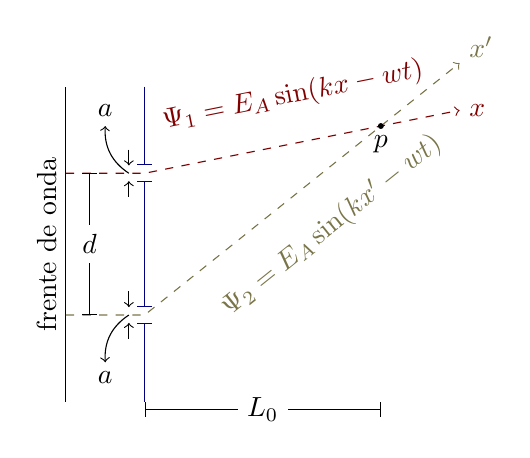
\begin{tikzpicture}
        \draw(0,-2) -- (0,2) node[midway, above, sloped] {frente de onda};

        % ~~~~ Rendijas ~~~~%
        \draw[color=blue!50!black,draw opacity=2, -| ] (1,2) -- (1,1);
        \draw[color=blue!50!black,draw opacity=2, |-| ] (1,0.8) -- (1,-0.8);
        \draw[color=blue!50!black,draw opacity=2, -| ] (1,-2) -- (1,-1);


        % ~~~~ Rayos y emisores ~~~~%
        \draw[color=red!50!black,dashed, ->] (0,0.9) -- (1,0.9) --
            node[midway, yshift=6mm, sloped] 
            {$\Psi_1 = E_A \sin(kx - wt)$} (5,1.7) node[right] {$x$};
        \draw[color=yellow!40!black,dashed, ->] (0,-0.9) -- (1,-0.9) --
            node[midway, yshift=-6mm, sloped]
            {$\Psi_2 = E_A \sin(kx' - wt)$} (5,2.3) 
            node[right,yshift=2mm] {$x'$};
        \filldraw (4,1.5) circle (0.3mm) node [below] {$p$};
        
        % ~~~~ Datos ~~~~ %
        \draw[|-|] (0.3,0.9) -- (0.3,-0.9) node[midway, fill=white]{$d$};
        \draw[ -> ] (0.8,0.6) -- (0.8,0.8);
        \draw[ -> ] (0.8,1.2) -- (0.8,1);
        \draw[ -> ] (0.8,0.9) to [bend left] (0.5, 1.5) node[above] {$a$};
        \draw[ -> ] (0.8,-0.6) -- (0.8,-0.8);
        \draw[ -> ] (0.8,-1.2) -- (0.8,-1);
        \draw[ -> ] (0.8,-0.9) to [bend right] (0.5, -1.5) node[below] {$a$};

        \draw[|-|] (1,-2.1) -- (4,-2.1) node[midway, fill=white] {$L_0$};
    \end{tikzpicture}
\end{center}

El efecto neto en $p$ es la suma de los efectos individuales. Esto es,
\[\Psi(p) = \Psi_1 + \Psi_2 = E_A \sin(kx - wt) + E_A \sin(kx' - wt)\]

Una condición del experimento, es que $L_0$ sea mucho mayor a $d$, que
a su vez es mucho mayor que $a$. Bajo esta condición, se pueden
aproximar las pendientes de ambos rayos, es decir, son paralelos.

\begin{center}
    \begin{tikzpicture}
        \draw (0,1) -- (0,-1) node[midway, left] {$d$};
        \draw[dashed, ->, color=red!50!black] (0,0.75) -- (2,1.75) 
            node[midway, above, sloped] {$\Psi_1$};
        \draw[dashed, ->, color=yellow!40!black] (0,-0.75) -- (2,0.25) 
            node[midway, below, sloped] {$\Psi_2$};

        \draw[dotted] (0,0.75) -- (1,0.75);
        \draw[dotted] (0,0.75) -- (0.6,-0.45);

        % ~~~~ coordenadas  ~~~~ %
        \coordinate (A) at (0.5,0.75);
        \coordinate (B) at (0,0.75);
        \coordinate (C) at (0.4,0.95);
        
        
        \coordinate (D) at (0,0);
        \coordinate (E) at (0,0.75);
        \coordinate (F) at (0.025,0.7);

        \coordinate (G) at (0,-0.75);
        \coordinate (H) at (0.6,-0.45);

        \pic [draw, "$\theta$", angle eccentricity=1.5] {angle = A--B--C};
        \pic [draw, "$\theta$", angle eccentricity=1.5] {angle = D--E--F};

        \draw[|-|] ([shift=(290:2mm)] G) -- ([shift=(290:2mm)] H)
            node[midway, fill=white, inner sep = 1pt, sloped] {$\delta$};
        
    \end{tikzpicture}
\end{center}
\[
    \begin{derivation}
            \res{ \delta = d\,\sin(\theta) }\\
        \To\\
            \res{ x' \approx x + \delta }\\
        \To\\
            \res{ \Psi(p) = E_A\sin(kx-wt) + E_A\sin(k(x+\delta) - wt) }\\
        \equiv\\
            \res{ \Psi(p) = E_A\sin(kx-wt) + E_A\sin(kx - wt + k\delta) }
    \end{derivation}
\]

Ahora, si consideramos el efecto neto en diferentes puntos, del frente
de onda en el que se encuentra $p$, los cuales tienen un valor $\delta$
asosiado, se puede deducir gran parte del efecto de interferencia en
dichos puntos:

\begin{enumerate}
    \item Sea $n \in \mathbb{N}$. Tomando $k\delta = (2n + 1)\pi$
    \[
        \begin{derivation}
                \res{ \Psi(p) = E_A\sin(kx - wt) + E_A\sin(kx - wt + k\delta) }\\
            \equiv\\
                \res{ \Psi(p) = E_A\sin(kx - wt) + E_A\sin(-(kx - wt))}\\
            \equiv\\
                \res{ \Psi(p) = E_A\sin(lx-wt) - E_A\sin(kx - wt) }\\
            \equiv\\
                \res{\Psi(p) = 0}
        \end{derivation}  
    \]
    Este caso se conoce como condición de interferencia destructiva (CID).

    Como $k = \dfrac{2\pi}{\lambda}$, entonces,
    $d\,\sin(\theta) = \left(n + \dfrac{1}{2}\right)\lambda$
    \item Sea $n \in \mathbb{N}$. Tomando $k\delta = 2n\pi$
    \[
        \begin{derivation}
                \res{ \Psi(p) = E_A\sin(kx - wt) + E_A\sin(kx - wt + k\delta) }\\
            \equiv\\
                \res{ \Psi(p) = E_A\sin(kx - wt) + E_A\sin(kx - wt) }\\
            \equiv\\
                \res{ \Psi(p) = 2E_A\sin(kx - wt) }
        \end{derivation}
    \]
    Este caso se conoce como condición de interferencia constructiva (CIC).

    Como $k = \dfrac{2\pi}{\lambda}$, entonces,
    $d\,\sin(\theta) = n\lambda$
\end{enumerate}

Volviendo al efecto neto en el punto $p$, esta expresión se puede
reescribir de la siguiente manera:

\[
    \begin{derivation}<2>[5pt]
            \res{  \Psi(p) = E_A\sin(kx - wt) + E_A\sin(kx - wt + k\delta) }\\
        \why{ $\sin(\alpha) + \sin(\beta) 
                = 2\cos\left(\dfrac{\alpha - \beta}{2}\right)
                \sin\left(\dfrac{\alpha+\beta}{2}\right)$ }\\
            \res{  \Psi(p) = 
                2E_A\cos\left(\frac{k\delta}{2}\right)
                    \sin\left(-wt + kx + \frac{k\delta}{2}\right) }\\
            \why{ $\gamma = kx + \dfrac{k\delta}{2} + \pi$}\\
                \res{ \Psi(p) =  2E_A\cos\left(\frac{k\delta}{2}\right)
                        \sin(wt + \gamma) }
    \end{derivation}
\]

Esta expresión, no es otra que la de una onda armónica simple. Esto nos
dice que el campo eléctrico oscila armónicamente con amplitud
$A(\delta) = 2E_A\cos\left(\dfrac{k\delta}{2}\right)$. Lo mismo ocurre
con el campo magnético $B$.
